


\section{Auswertung}

\section{Auswertung}

\subsection{Filterkurve des Selektivverstärkers}
In \autoref{tab:filterkurve} befinden sich die gemessenen Spannungen $\frac{U_{A}}{U_{E}}$ in Abhängigkeit zur Frequenz $\nu$.
\begin{table}[H]
 \centering 
 \captionabove{Spannungen in Abhängigkeit zur Frequenz}
 \begin{tabular}{l|l|l|l} 
 $\nu$ [kHz]& $\frac{U_{A}}{U_{E}}$ [mV] & $\nu$ [kHz]& $\frac{U_{A}}{U_{E}}$ [mV]\\  \hline
 20.6 & 190 & 33.6 & 2000\\ 
 21.4 & 210 & 34.1 & 2500\\ 
 22   & 220 & 35   & 6900\\
 23.3 & 250 & 36.5 & 4000\\
 24.1 & 280 & 37.2 & 1500\\
 25.6 & 300 & 38.1 & 1200\\
 26.2 & 350 & 39.4 & 900\\
 27   & 430 & 40.2 & 700\\
 28   & 500 & 41.1 & 670\\
 29.4 & 630 & 42   & 600\\
 30.3 & 680 & 43.5 & 490\\
 31.1 & 940 & 44.1 & 430\\
 32.3 & 1100 & 45.2 & 400\\ \hline
 \end{tabular} 
 \label{tab:filterkurve}
\end{table} 
Die Werte aus \autoref{tab:filterkurve} können in eine Gaußfunktion $U(\nu)=a\cdot exp(-(\frac{\nu-b}{c})^2)$ gefittet werden. 
Unter der Benutzung von Matlab ergeben sich für die Parameter $a=7152\ \si{\V}$, $b=35.42$ kHz und $c=1.467$ kHz, 
mit der maximalen Spannung von $U_{max}=7152\ \si{\V}=a$ bei der Frequenz $\nu_{0}=35.42\ \si{\kHz}=b$. 
Die Frequenzen $\nu_{+}$ und $\nu_{-}$ können durch die Beziehung $U(\nu)=\frac{1}{\sqrt{2}}$ berechnet werden. 
Somit ergibt sich für $\nu_{+}=39.875$ und für $\nu_{-}=30.965$. 
Aus $\nu_{0}$, $\nu_{+}$ und $\nu_{-}$ lässt sich die Güte mithilfe von \autoref{eq:guetekuh}
berechnen. Es ergibt sich eine Güte von $Q=3.975$.
\begin{figure}[H]
  \centering
  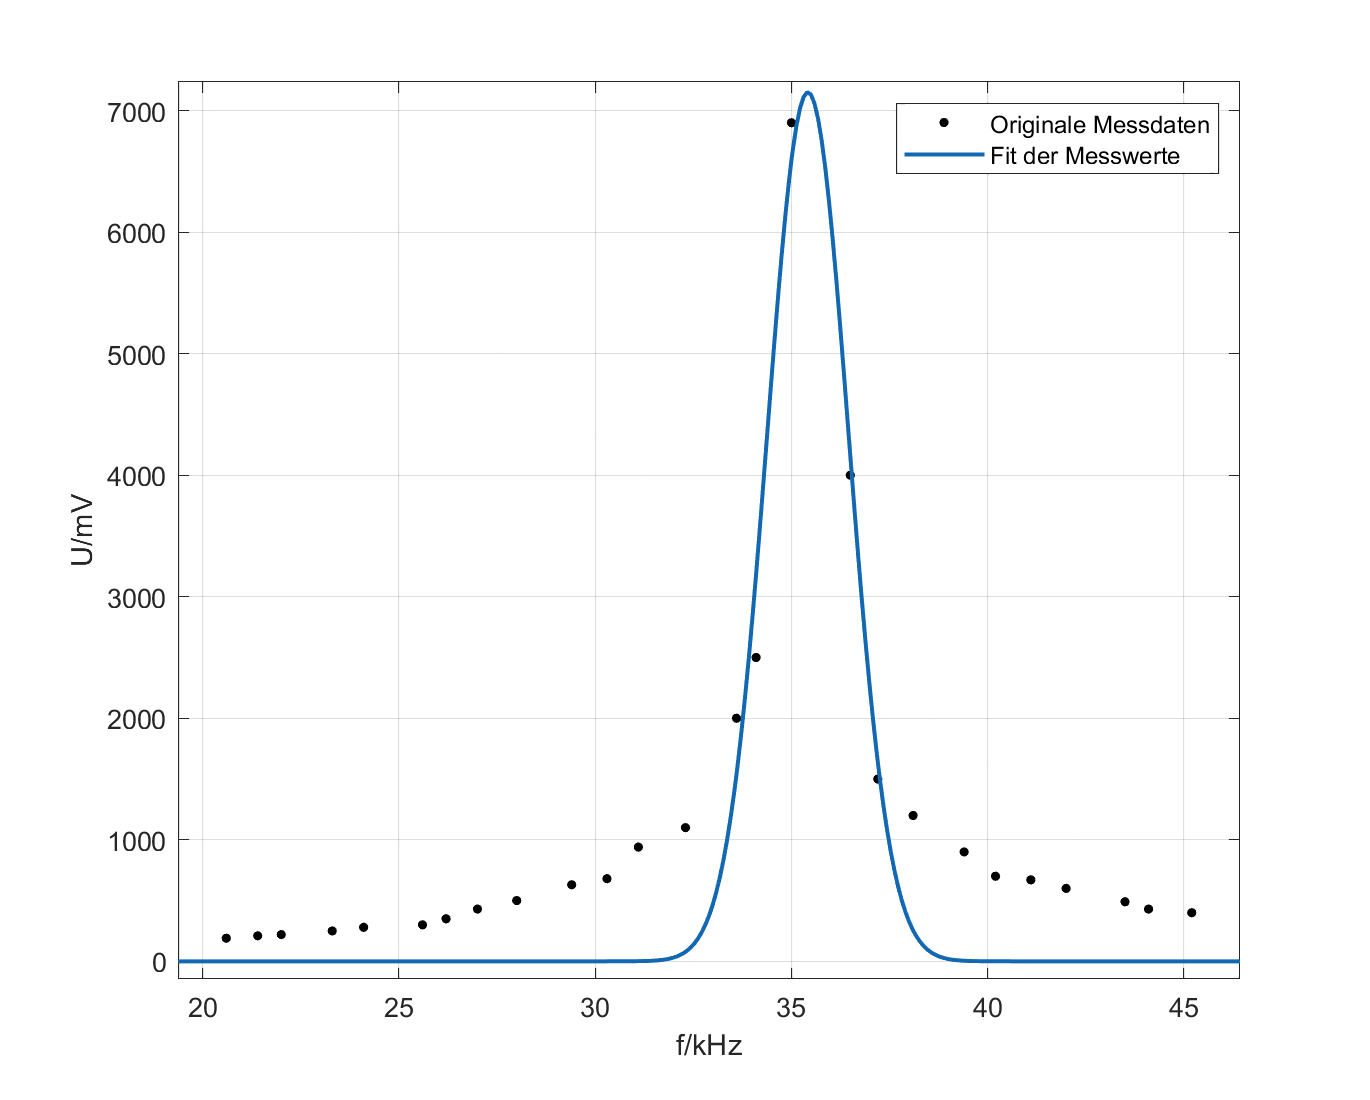
\includegraphics[width=12cm]{fit.png}
  \caption{Fit der Messdaten auf eine Gaußfunktion.}
\end{figure}

\subsection{Suszeptibilitäten seltener Erden}
Für den Versuch wurden die Suszeptibilitäten der drei Stoffe $Nd_2 O_3$, $Dy_2 O_3$ und $Gd_2 O_3$ überprüft. Dazu wurde einer Spannung von $1$ V eingespeist. In \autoref{tab:2} befinden sich die niedrigsten Brückenspannungen und Widerstände mit und ohne seltener Erde.
\begin{table}[H]
  \centering
  \caption{Gemessene Spannungen und Widerstände.}
  \begin{tabular}{l|l|l|l|l}
  & $U_{o}$ [mV] & $U_{m}$ [mV] & $R_{o}$ [$\Omega$] & $R_{a}$ [$\Omega$]\\ \hline
  $Nd_2 O_3$ & 300 & 300 & 704 & 667\\
  & 279 & 279 & 708 & 665\\
  & 980 & 990 & 675 & 713\\ \hline
  $Dy_2 O_3$ & 990 & 330 & 670 & 478\\
  & 990 & 330 & 687 & 475\\
  & 990 & 300 & 716 & 472\\ \hline
  $Gd_2 O_3$ & 970 & 1000 & 703 & 588\\
  & 970 & 990 & 697 & 590\\
  & 980 & 990 & 675 & 596\\ \hline
  \end{tabular}
  \label{tab:2}
\end{table}
Die wichtigsten Größen der Stoffe sind \autoref{tab:3} zu entnehmen,
\begin{table}[H]
  \centering
  \caption{Die wichtigsten Größen der drei Stoffe.}
  \begin{tabular}{l|l|l|l|l|l}
  & m [$\mathrm{g}$] & M [$\mathrm{g/mol}$] & $\rho$ [$\mathrm{g/cm^3}$] & L [$\mathrm{cm}$] & Q [$\mathrm{m^2}$]\\ \hline
  $Nd_2 O_3$ & 18.48 & 336.48 & 7.24 & 15.3 & 1.668$\cdot$10$^{-5}$ \\ \hline
  $Dy_2 O_3$ & 15.10 & 373 & 7.8 & 15.2 & 1.27$\cdot$10$^{-5}$ \\ \hline
  $Gd_2 O_3$ & 14.68 & 363 & 7.4 & 15.3 & 1.30$\cdot$10$^{-5}$ \\ \hline
  \end{tabular}
  \label{tab:3}
\end{table}
wobei sich der Querschnitt Q der Probe aus 
\begin{equation*}
  Q=\frac{m}{L\rho}
\end{equation*}
berechnen lässt, m die Masse, M die molare Masse, $\rho$ die Dichte und L die Länge der Probe ist.
Aus den gemessenen Werten ergeben sich die folgenden aufgelisteten mittleren Widerstandsdifferenzen
\begin{align*}
  \bar R_{Nd_2 O_3}&=(0.197 \pm 0.009) \si{\ohm},\\
  \bar R_{Dy_2 O_3}&=(1.083 \pm 0.076) \si{\ohm}\ \textrm{und}\\
  \bar R_{Gd_2 O_3}&=(0.502 \pm 0.055) \si{\ohm}
\end{align*}
aus den Formeln
\begin{equation*}
  \bar A=\frac{1}{n}\sum_{i=1}^n A_i
  \label{eq:fehler}
\end{equation*}
\begin{equation*}
  \Delta A=\sqrt{\frac{1}{n(n-1)}\sum_{i=1}^n (A_i - \bar A)^2},
\end{equation*}
wobei A eine beliebige Größe ist, dessen Mittelwert und Fehler ausgerechnet werden soll und n die Anzahl an Messungen dieser Größe.\\
Aus diesen Mittelwerten ergeben sich mit \autoref{eq:alternativ} und    
\begin{equation}
  \Delta f(A)=\sqrt{\left(\frac{\partial f(A)}{\partial A}\right)^2 (\Delta A)^2}
  \label{gauß}
\end{equation}
die Suszeptibilitäten 
\begin{align*}
  \bar \chi_{Nd_2 O_3}&=(0.00204 \pm 0.00009),\\
  \bar \chi_{Dy_2 O_3}&=(0.0148 \pm 0.0010)\ \textrm{und}\\
  \bar \chi_{Gd_2 O_3}&=(0.0067 \pm 0.0007)
\end{align*}
der seltenen Erden.\\
Über \eqref{eq:1} ergibt sich 
\begin{align*}
  \bar \chi_{Nd_2 O_3}&=(0.194 \pm 3547.80),\\
  \bar \chi_{Dy_2 O_3}&=(18.27 \pm 87.28)\ \textrm{und}\\
  \bar \chi_{Gd_2 O_3}&=(0.542 \pm 123.38)
\end{align*}
für die Suszeptibilitäten. Dabei wurden die drei Spannungen $U_{o}$ und $U_{m}$ aus \autoref{tab:2} pro Stoff mit \autoref{fehler} gemittelt und in \eqref{eq:1} eingesetzt. Dabei ergaben sich die Brücken- und Erregerspannungen
\begin{align*}
  \bar U_{Br_{Nd_2 O_3}}&=(519.67 \pm 230.25) \textrm{mV},\\
  \bar U_{err_{Nd_2 O_3}}&=(529 \pm 230.50) \textrm{mV},\\
  \bar U_{Br_{Dy_2 O_3}}&=(990 \pm 0) \textrm{mV},\\
  \bar U_{err_{Br_{Dy_2 O_3}}}&=(320 \pm 10) \textrm{mV},\\
  \bar U_{Br_{Gd_2 O_3}}&=(973 \pm 3.33) \textrm{mV}\ \textrm{und}\\
  \bar U_{err_{Br_{Gd_2 O_3}}}&=(993.33 \pm 3.33) \textrm{mV}
\end{align*}
für die Stoffe.\\
Die theoretischen Werte können durch die Hundschen Regeln berechnet werden. Dazu werden der Gesamtdrehimpuls J, der Spin S, der Bahndrehimpuls L und der gyromagnetische Faktor $g_j$ des Moleküls benötigt. Diese sind für die drei Stoffe in \autoref{tab:4} gelistet.
\begin{table}[H]
  \centering
  \caption{Drehimpulse und gyromagnetischer Faktor der einzelnen Stoffe.}
  \begin{tabular}{l|l|l|l|l}
   & J & S & L & $g_j$\\ \hline
   $Nd_2 O_3$ & 9/2 & 3/2 & 6 & 0.72\\ \hline
   $Dy_2 O_3$ & 15/2 & 5/2 & 5 & 1.33\\ \hline
   $Gd_2 O_3$ & 7/2 & 7/2 & 0 & 2\\ \hline
   \end{tabular}
   \label{tab:4}
\end{table}
wobei sich das gyromagnetische Verhältnis aus \autoref{eq:gyromyro} berechnet. 
Wird alles in \autoref{eq:sus} eingesetzt, ergibt sich für die theoretischen Suszeptibilitäten
\begin{align*}
  \chi_{th_{Nd_2 O_3}}&=0.00296\\
  \chi_{th_{Dy_2 O_3}}&=0.02530\\
  \chi_{th_{Gd_2 O_3}}&=0.01377
\end{align*}
wenn für N % aus \eqref{8} --- ist gar nicht in der theorie ---
\begin{equation*}
  N=\frac{Z\rho}{M}\cdot N_{A}
\end{equation*}
genutzt wird, wobei M die molare Masse des Stoffes, $\rho$ die Dichte des Stoffes, $N_A$ die Avogadro-Zahl ist. Für alle Stoffe gilt $Z=2$.
